% !TEX TS-program = pdflatex
% !TEX encoding = UTF-8 Unicode

% This is a simple template for a LaTeX document using the "article" class.
% See "book", "report", "letter" for other types of document.

\documentclass[11pt]{article} % use larger type; default would be 10pt

\usepackage[utf8]{inputenc} % set input encoding (not needed with XeLaTeX)

%%% Examples of Article customizations
% These packages are optional, depending whether you want the features they provide.
% See the LaTeX Companion or other references for full information.

%%% PAGE DIMENSIONS
\usepackage{geometry} % to change the page dimensions
\geometry{letterpaper} % or letterpaper (US) or a5paper or....
% \geometry{margin=2in} % for example, change the margins to 2 inches all round
% \geometry{landscape} % set up the page for landscape
%   read geometry.pdf for detailed page layout information

\usepackage{graphicx} % support the \includegraphics command and options
\graphicspath{ {./images/} }

% \usepackage[parfill]{parskip} % Activate to begin paragraphs with an empty line rather than an indent

%%% PACKAGES
\usepackage{booktabs} % for much better looking tables
\usepackage{array} % for better arrays (eg matrices) in maths
\usepackage{paralist} % very flexible & customisable lists (eg. enumerate/itemize, etc.)
\usepackage{verbatim} % adds environment for commenting out blocks of text & for better verbatim
\usepackage{subfig} % make it possible to include more than one captioned figure/table in a single float
% These packages are all incorporated in the memoir class to one degree or another...

\usepackage{siunitx}
\usepackage{hyperref}

%%% HEADERS & FOOTERS
\usepackage{fancyhdr} % This should be set AFTER setting up the page geometry
\pagestyle{fancy} % options: empty , plain , fancy
\renewcommand{\headrulewidth}{0pt} % customise the layout...
\lhead{}\chead{}\rhead{}
\lfoot{}\cfoot{\thepage}\rfoot{}

%%% SECTION TITLE APPEARANCE
\usepackage{sectsty}
\allsectionsfont{\sffamily\mdseries\upshape} % (See the fntguide.pdf for font help)
% (This matches ConTeXt defaults)

%%% ToC (table of contents) APPEARANCE
\usepackage[nottoc,notlof,notlot]{tocbibind} % Put the bibliography in the ToC
\usepackage[titles,subfigure]{tocloft} % Alter the style of the Table of Contents
\renewcommand{\cftsecfont}{\rmfamily\mdseries\upshape}
\renewcommand{\cftsecpagefont}{\rmfamily\mdseries\upshape} % No bold!

%%% END Article customizations

%%% The "real" document content comes below...

\title{Simulink Model of PID + FOC for BLDC}
\author{Andy Berger}
%\date{} % Activate to display a given date or no date (if empty),
         % otherwise the current date is printed 

\begin{document}
\maketitle

\section{Motor Model}

\begin{figure}
\centering
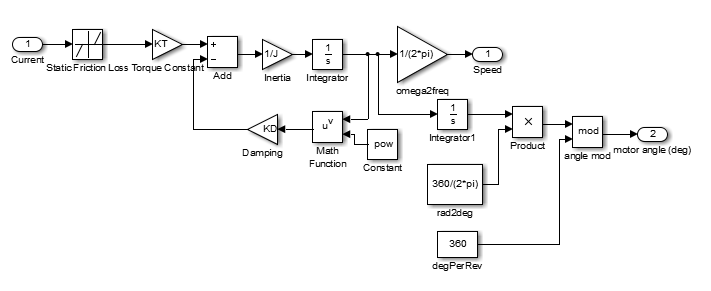
\includegraphics[scale=0.75]{BLDCblockDiagram.png}
\caption{Simulink block diagram for BLDC motor}
\label{fig:BLDCblockDiagram}
\end{figure}

The motor model (Fig. \ref{fig:BLDCblockDiagram}) is based on the transfer function:
\begin{equation}
\Omega(s) = \frac{K_T}{J s + K_D} I_Q(s)
\end{equation}
\noindent where $\omega$ is the motor frequency, $K_T$ is the torque constant (in \si{N.m/A}), $J$ is the moment of inertia (in \si{kg.m^2}), $K_D$ is the damping constant (in \si{N.m/Hz}), and $I_Q$ is the current applied to the Q-axis (in the D-Q reference frame, the Q-axis is responsible for the torque applied to the rotor moment).

From impulse response measurements [include figure], the minimum current necessary to start the motor spinning from rest is about 0.05 A (see Fig. \ref{fig:accelVsCurrent}). This is used with the Static Friction Loss block. 
\begin{figure}
\centering
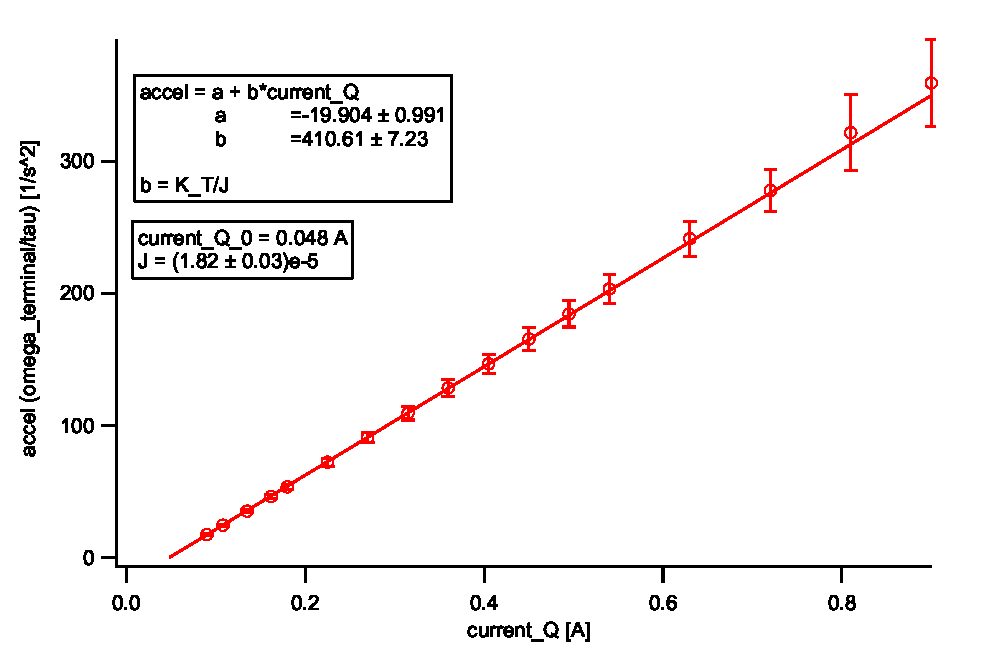
\includegraphics[scale=0.75]{accelVsCurrent.eps}
\caption{Acceleration vs. applied current\_Q for Elinco 16 mm motor}
\label{fig:accelVsCurrent}
\end{figure}

I can convert the Laplace-domain transfer function for $\Omega(s)$ to a time-domain solution using the following general solution [http://lpsa.swarthmore.edu/Transient/TransInputs/TransStep.html]: 
\begin{equation}
y(t) = H(0) + [H(\infty) - H(0)]\exp(-t/\tau)
\end{equation}

\begin{equation}
\omega(t) = \frac{K_T I_Q}{K_D} \left(1 - \exp(-t/\tau)\right)
\end{equation}
\noindent where $\tau \equiv J/K_D$ (note that the inverse Laplace transform of $1/(s + a)$ is $\exp(-a t)$). Also, define $\omega_f \equiv K_T I_Q/K_D$. So fitting the time response $\omega(t)$ as a function of time, acquired from impulse response tests [include figure], I can extract $\omega_f$ (the terminal frequency as $t \rightarrow \infty$). A plot of $\omega_f/\tau$ vs applied current will have a slope given by $K_T/J$. The torque constant used for the simulations is provided in the spec sheet of the motor: \SI{7.5}{mN.m/A}. Therefore, I can extract the moment of inertia $J$ (see "impulse measurements (7-10-18).pxp").

There are a couple of ways to extract the damping constant $K_D$. Using the definition of the motor time constant, I can assume that the motor damping has a frequency dependence of the form:

\begin{equation}
\tau = \frac{J}{K_{D,0} (\omega_f)^x}
\end{equation}

\noindent that is, the total damping torque (at terminal velocity) is given by $N_D = K_{D,0} (\omega_f)^x$. Then, by plotting $\log(\tau)$ vs. $\log(\omega_f)$, I can extract both $K_{D,0}$ (assuming $J$ has already been determined) and $x$.

\begin{equation}
\log(\tau) = \log\left(\frac{J}{K_{D,0}}\right) - x \log(\omega_f)
\end{equation}

Alternatively, from the definition of $\omega_f$, I can re-arrange:
\begin{equation}
I_Q = \frac{K_{D,0} (\omega_f)^x}{K_T}
\end{equation}

\noindent a similar log-log analysis yields:
\begin{equation}
\log(I_Q) = \log\left(\frac{K_{D,0}}{K_T}\right) + x \log(\omega_f)
\end{equation}

\noindent From these two methods, I find $x \approx 1.88$. \textbf{How was $K_{D,0}$ determined?}

A summary of the motor parameters needed for the Simulink model are presented in Tab. \ref{tab:MotorParams}.
\begin{table}
\centering
\begin{tabular}{l | l}
\textbf{Parameter} & \textbf{Value} \\
$J$ & \SI{1.66e-5}{kg.m^2} \\
$K_D$ & \SI{1.95e-9}{} \\
$K_T$ & \SI{7.5}{mN.m/A} \\
$x$ & 1.88
\end{tabular}
\caption{Motor parameters that must be initialized to run Simulink model}
\label{tab:MotorParams}
\end{table}

\section{Closed-Loop Speed and Phase Control}

\begin{figure}
\centering
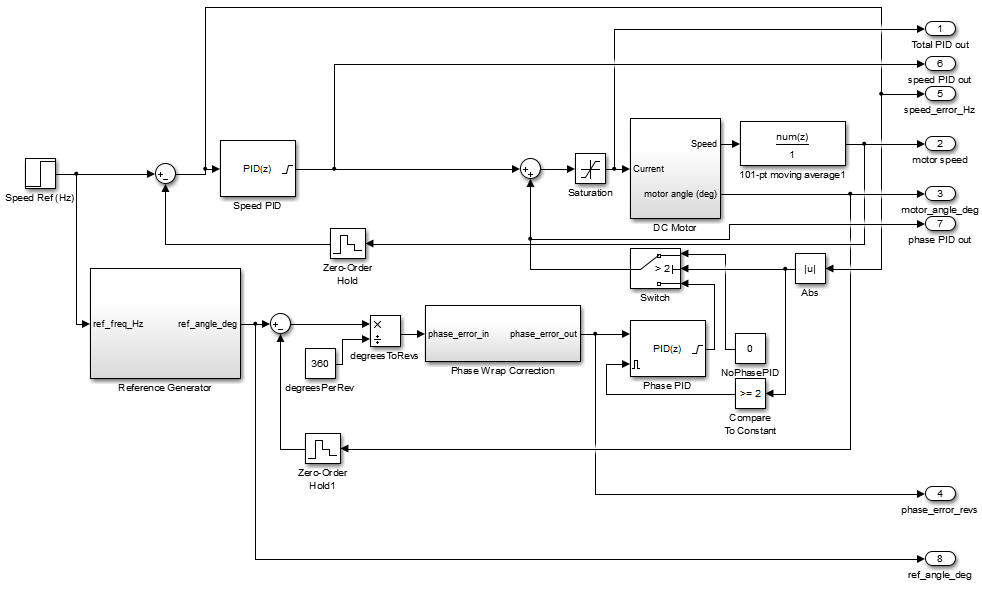
\includegraphics[scale=0.75,angle=90,origin=c]{MotorPIDBlockDiagram.png}
\caption{Simulink block diagram for closed loop speed and phase control of DC motor}
\label{fig:BLDCblockDiagram}
\end{figure}

To simulate closed-loop operation of the motor, a speed reference is provided by a step function source block. From the speed reference, the speed error is calculated and fed to the speed PID. 

\begin{table}[h]
\centering
\begin{tabular}{l | l }
\textbf{Controller Parameter} & \textbf{Value} \\
P & 0.1 \\
I & 0 \\
D & 0 \\
\end{tabular}
\caption{Speed PID coefficients}
\label{tab:SpeedPIDcoeffs}
\end{table}

The speed reference is also converted to a phase by the "Reference Generator" block. This simply integrates the speed, and then performs a modulo operation to convert the integrated speed to a phase angle in degrees. The phase error is calculated and then sent to the "Phase Wrap Correction" which makes sure that the phase error is defined on the domain [-0.5, 0.5) (in revs). This phase wrapped error is fed to the Phase PID block.

\begin{table}[h]
\centering
\begin{tabular}{l | l }
\textbf{Controller Parameter} & \textbf{Value} \\
P & 0.5 \\
I & 0.5 \\
D & 0.1 \\
Filter Coefficient (N) & 100
\end{tabular}
\caption{Phase PID coefficients}
\label{tab:PhasePIDcoeffs}
\end{table}

\noindent An external reset input is fed by the speed error. This resets the integral phase error anytime the speed error is greater than some threshold (speed\_thres (Hz)). Otherwise, the integral phase error can easily wind up during time periods when the motor is far from speed lock, causing a wind-up condition that is difficult to escape. Finally, whether the phase PID output is added to the speed PID output is determined by the same speed\_thresh criteria. That is, if the speed error is too large, the phase PID output is not used to servo the motor current.

The motor block provides speed and angle outputs for use with the closed loop feedback. The speed is averaged over 101 points as a rudimentary low-pass filter.

Zero-Order Holds are used for the motor speed and phase to represent the digital sampling of these quantities by the MCU.

\section{Closed Loop PID model}
\begin{equation}
\frac{K_T K_d s^2 + K_T K_p s + K_T K_i } {J s^3 + K_D s^2 + K_T K_d s^2 + K_T K_p s + K_T K_i}
\end{equation}

\end{document}
